% !TEX root = Slide_Presentasi_DWBI_Healthcare_v2.tex

%=============================================================
% SLIDE PRESENTASI: DWBI HEALTHCARE  (v2 – fixes)
%=============================================================

\documentclass[xcolor=table,t,aspectratio=169]{beamer}
\usepackage{pgfpages,graphicx,listings,hyperref}
\usepackage[table]{xcolor}
\usepackage{multicol,multirow}
\usepackage{listings}
\usepackage{tikz}
\usetikzlibrary{positioning,arrows.meta,shapes}
\usepackage{tcolorbox}
\tcbuselibrary{skins}
\usepackage{booktabs}
\usepackage{tabularx}
\usepackage{array}
\usepackage{enumerate}
\usepackage[utf8]{inputenc}
\usepackage[T1]{fontenc}
\usepackage{amsmath}

\definecolor{ugmyellow}{HTML}{f6d648}
\definecolor{ugmblue}{HTML}{194168}
\definecolor{ugmbackgroundblue}{HTML}{00416B}
\definecolor{ugmbackgroundgrey}{RGB}{220,220,220}
\definecolor{ugmgray}{HTML}{E0E0E0}
\definecolor{codegreen}{rgb}{0,0.6,0}
\definecolor{codegray}{rgb}{0.5,0.5,0.5}
\definecolor{backcolour}{rgb}{0.95,0.95,0.92}

\lstset{
  basicstyle=\ttfamily\tiny,
  breaklines=true,
  frame=single,
  backgroundcolor=\color{backcolour},
  keywordstyle=\color{ugmblue}\bfseries,
  commentstyle=\color{codegreen},
  stringstyle=\color{red},
  showstringspaces=false,
  numbers=left,
  numberstyle=\tiny\color{codegray},
  stepnumber=1,
  numbersep=5pt
}

\renewcommand{\figurename}{Gambar}
\newcommand{\teksmerah}[1]{{\color{red} #1}}
\newcommand{\teksbiru}[1]{{\color{ugmblue} #1}}
\newcommand{\tekshijau}[1]{{\color{green!60!black} #1}}

\tcbset{
  kontribbox/.style={
    enhanced,
    colback=ugmblue!8,
    colframe=ugmblue,
    colbacktitle=ugmblue,
    coltitle=white,
    fonttitle=\small\bfseries\ttfamily,
    attach boxed title to top left={yshift=-2mm, xshift=4mm},
    boxed title style={sharp corners, colback=ugmblue, colframe=ugmblue},
    sharp corners=south,
    top=4pt, bottom=4pt, left=6pt, right=6pt,
  }
}

\hypersetup{%
  pdftitle={DWBI Healthcare - Multidimensional Modeling},%
  pdfauthor={Engelbertus Rande, Gilbert Fandiliam Mooy, Sinta Siti Nuriah, Vicky Mahfudy},%
  pdfsubject={Tugas Kelompok Data Warehouse and Business Intelligence},%
  pdfkeywords={Data Warehouse, OLAP, Star Schema, dbt, Airflow, Healthcare}%
}
\definecolor{links}{HTML}{2A1B81}
\hypersetup{colorlinks,linkcolor=,urlcolor=links}
\setbeamercovered{transparent}

\title[DWBI Healthcare]{Multidimensional Modeling\\untuk Sistem DWBI Healthcare}
\subtitle{Tugas Kelompok: Data Warehouse and Business Intelligence}

\author[Kelompok Healthcare]{%
  Engelbertus Rande\inst{1} \and
  Gilbert Fandiliam Mooy\inst{2} \and
  Sinta Siti Nuriah\inst{3} \and
  Vicky Mahfudy\inst{4}%
}

\institute[UGM]{%
  \inst{1} NIM 25/573149/PPA/07211 \quad
  \inst{2} NIM 25/574767/PPA/07259 \\[2pt]
  \inst{3} NIM 25/575177/PPA/07274 \quad
  \inst{4} NIM 25/573019/PPA/07207 \\[4pt]
  Program Studi S2 Ilmu Komputer, Universitas Gadjah Mada\\
  Dosen: Khabib Mustofa%
}

\date{Mei 2026}

\usefonttheme{professionalfonts}
\setbeamerfont{title}{series=\bfseries,parent=structure}
\setbeamerfont{frametitle}{series=\bfseries,parent=structure}

\mode<presentation>{ \logo{
\includegraphics[height=.75cm]{images/logougm.png}} }

\usetheme{Copenhagen}
\usecolortheme{seahorse}
\setbeamertemplate{headline}{}

\setbeamercolor{title}{bg=ugmgray, fg=ugmblue}
\setbeamercolor{frametitle}{bg=white, fg=ugmblue}
\setbeamercolor{section in head/foot}{fg=white, bg=ugmblue}
\setbeamercolor{subsection in head/foot}{fg=black, bg=ugmgray}
\setbeamertemplate{blocks}[rounded]
\setbeamercolor{block title}{fg=white, bg=ugmblue}
\setbeamercolor{block body}{fg=black, bg=ugmblue!8}

\setbeamertemplate{footline}{
  \leavevmode%
  \hbox{%
    \colorbox{ugmgray}{\makebox[.50\paperwidth][l]{\color{ugmblue}\hspace{2ex}
      \usebeamerfont{author in head/foot}
      \textbf{Merakyat, Mandiri, Berkelanjutan $|$ Inclusive, Self-Reliant, Sustainable}
    }}%
    \colorbox{ugmbackgroundblue}{\makebox[.15\paperwidth][c]{
      \color{white}\usebeamerfont{title in head/foot}\textbf{ugm.ac.id}
    }}%
    \colorbox{ugmgray}{\makebox[.40\paperwidth][c]{
      \color{black}\usebeamerfont{date in head/foot}
      \textbf{\insertshorttitle\ (\insertframenumber/\inserttotalframenumber) \hspace{2ex}}
    }}
  }%
  \vskip0pt%
}

\usebackgroundtemplate{%
  \tikz\node[opacity=0.2]{
\includegraphics[height=\paperheight]{images/latar31.jpg}};%
}

\setbeamertemplate{caption}[numbered]

\AtBeginSection[]
{
  \begin{frame}{Cakupan Materi}
    \footnotesize
    \tableofcontents[currentsection]
  \end{frame}
}

%=============================================================
\begin{document}
%=============================================================

\frame{\titlepage}

\begin{frame}{Daftar Isi}
  \footnotesize
  \tableofcontents
\end{frame}

%=============================================================
%  SLIDE KONTRIBUSI GITHUB  (1/2)
%=============================================================
\begin{frame}{Kontribusi Tim -- Bagian 1/2}
  \footnotesize
  \textbf{Repository:}
  \href{https://github.com/vickymahfudy/dwbi-healthcare}%
       {\texttt{github.com/vickymahfudy/dwbi-healthcare}}
  \vspace{6pt}

  \begin{columns}[T]
    \column{0.48\textwidth}
    \begin{tcolorbox}[kontribbox, title={\texttt{vickymahfudy} (Vicky Mahfudy)}]
      \scriptsize
      \begin{itemize}\itemsep1pt
        \item Inisiasi repositori dan struktur proyek
        \item Setup Apache Airflow di Docker
        \item Pengembangan data generator dengan \textit{Faker} (branch \texttt{faker-data})
        \item Koneksi pipeline ke PostgreSQL
        \item Penambahan \texttt{dbt run} \& \texttt{dbt test} ke DAG
        \item Rename DAG dan resolusi konflik Airflow
        \item Merge PR \#1 (faker-data) dan PR \#2 (main)
        \item Update dokumentasi README
      \end{itemize}
    \end{tcolorbox}

    \column{0.48\textwidth}
    \begin{tcolorbox}[kontribbox, title={\texttt{Sintasitinuriah} (Sinta Siti Nuriah)}]
      \scriptsize
      \begin{itemize}\itemsep1pt
        \item Penambahan dataset awal ke repositori
        \item Penambahan konfigurasi multi-disease
        \item Penambahan dokumentasi dan pembaruan link
        \item Penambahan schema generator baru
        \item Konfigurasi dan penambahan DBT
        \item Resolusi merge conflict berulang
        \item Update README dan operasi merge branch
      \end{itemize}
    \end{tcolorbox}
  \end{columns}
\end{frame}

%=============================================================
%  SLIDE KONTRIBUSI GITHUB  (2/2)
%=============================================================
\begin{frame}{Kontribusi Tim -- Bagian 2/2}
  \footnotesize
  \textbf{Repository:}
  \href{https://github.com/vickymahfudy/dwbi-healthcare}%
       {\texttt{github.com/vickymahfudy/dwbi-healthcare}}
  \vspace{6pt}

  \begin{columns}[T]
    \column{0.48\textwidth}
    \begin{tcolorbox}[kontribbox, title={\texttt{ghost-45-max} (Engelbertus Rande)}]
      \scriptsize
      \begin{itemize}\itemsep1pt
        \item Penambahan 10.000 record ke dataset
        \item Implementasi DBT (\texttt{update implementasi DBT})
        \item Update manifest DBT
        \item Finalisasi implementasi DBT
        \item Konfigurasi Metabase (2 commit)
        \item Merge branch \texttt{main} dari GitHub
      \end{itemize}
    \end{tcolorbox}

    \column{0.48\textwidth}
    \begin{tcolorbox}[kontribbox, title={\texttt{masibeth} (Gilbert Fandiliam Mooy)}]
      \scriptsize
      \begin{itemize}\itemsep1pt
        \item Update modul requirements
        \item Revisi README (panduan virtual environment)
        \item Perbaikan konfigurasi YAML Docker Airflow
        \item Update referensi modul ajar (LaTeX)
        \item Perbaikan modul ajar: star diagram, Bab 5
        \item Perbaikan konfigurasi \texttt{schema.yml} DBT
        \item Perbaikan konflik kode LaTeX
        \item Force push update pipeline Airflow
        \item Revisi dan finalisasi modul ajar PDF
      \end{itemize}
    \end{tcolorbox}
  \end{columns}
\end{frame}

%=============================================================
%  BAB 1: PENDAHULUAN
%=============================================================
\section{Pendahuluan}

\begin{frame}{Domain dan Gambaran Dataset}
  \footnotesize
  \begin{columns}[T]
    \column{0.50\textwidth}
    \textbf{Domain: Healthcare (Operasional RS)}\\[4pt]
    Tiga pilar analisis utama:
    \begin{itemize}
      \item \textbf{Kunjungan Pasien} --- tipe fasilitas, Length of Stay, status keluar, metode pembayaran
      \item \textbf{Tenaga Medis} --- spesialisasi dokter, izin praktek (STR), biaya konsultasi
      \item \textbf{Rincian Biaya} --- konsultasi, obat, tindakan, kamar
    \end{itemize}

    \vspace{6pt}
    \begin{block}{Dataset Sintetis}
      \tiny
      \begin{tabular}{@{}ll@{}}
        \toprule
        \textbf{Aspek} & \textbf{Keterangan} \\
        \midrule
        Sumber           & 3 file CSV \\
        Total Kunjungan  & 12.000 baris \\
        Pasien           & 2.500 profil \\
        Dokter           & 80 master \\
        Rentang Waktu    & Jan 2025 -- Awal 2026 \\
        Fasilitas        & IGD, Rawat Jalan, Rawat Inap \\
        Pembayaran       & BPJS, Asuransi Swasta, Mandiri \\
        \bottomrule
      \end{tabular}
    \end{block}

    \column{0.48\textwidth}
    \textbf{Latar Belakang Masalah}
    \begin{enumerate}
      \scriptsize
      \item Data pasien, jadwal dokter, dan billing tersebar -- belum terintegrasi
      \item Belum ada infrastruktur DW dengan \textit{Star Schema}
      \item Keterbatasan pelacakan komponen biaya medis per fasilitas
      \item Keterbatasan akses data riil akibat regulasi privasi
    \end{enumerate}

    \vspace{6pt}
    \textbf{Tujuan Umum}\\[2pt]
    \scriptsize Membangun sistem DWBI operasional RS yang mengintegrasikan profil pasien, data master dokter, dan transaksi kunjungan ke dalam pemodelan dimensional untuk mendukung pengambilan keputusan klinis dan finansial.
  \end{columns}
\end{frame}

\begin{frame}{Tujuan Khusus}
  \footnotesize
  \begin{enumerate}
    \item \textbf{Integrasi Data} --- Menggabungkan 3 sumber heterogen (\texttt{source\_pasien.csv}, \texttt{source\_dokter.csv}, \texttt{source\_kunjungan.csv}) menjadi satu model terpadu (12.000 transaksi).
    \vspace{4pt}
    \item \textbf{Analisis Utilisasi} --- Menganalisis pola penggunaan fasilitas (rawat inap, rawat jalan, IGD) dan evaluasi efisiensi berbasis \textit{Length of Stay} (LOS).
    \vspace{4pt}
    \item \textbf{Analisis Finansial} --- Menganalisis distribusi pendapatan operasional berdasarkan komponen biaya, spesialisasi dokter, dan metode pembayaran.
    \vspace{4pt}
    \item \textbf{Pemodelan Dimensional} --- Membangun \textit{Star Schema} untuk kemudahan ekstraksi pelaporan OLAP tingkat lanjut.
    \vspace{4pt}
    \item \textbf{Data Sintetis} --- Menyediakan dataset berkualitas tinggi untuk pengembangan dan pengujian DWBI tanpa pelanggaran privasi pasien.
  \end{enumerate}
\end{frame}

%=============================================================
%  BAB 2: ANALISIS KEBUTUHAN BISNIS
%=============================================================
\section{Analisis Kebutuhan Bisnis}

\begin{frame}{Business Questions (BQ-01 s.d.\ BQ-06)}
  \scriptsize
  \begin{tabular}{cp{4.4cm}p{2.2cm}p{3.8cm}}
    \toprule
    \textbf{No} & \textbf{Business Question} & \textbf{Kategori} & \textbf{KPI / Metrik} \\
    \midrule
    1 & Total pendapatan dan distribusi per tipe fasilitas
      & Finansial & \texttt{SUM(total\_biaya)} per \texttt{tipe\_fasilitas} \\[2pt]
    2 & Spesialisasi dokter dengan volume transaksi dan total biaya terbesar
      & Kinerja Dokter & \texttt{COUNT}, \texttt{SUM(total\_biaya)} per spesialisasi \\[2pt]
    3 & Distribusi metode pembayaran (BPJS, Asuransi Swasta, Mandiri)
      & Finansial \& Payer & Persentase \texttt{total\_biaya} per metode \\[2pt]
    4 & Rata-rata \textit{Length of Stay} dan pengaruhnya terhadap biaya
      & Efisiensi Klinis & AVG(\texttt{lama\_rawat\_hari}), \texttt{biaya\_kamar} \\[2pt]
    5 & Tren bulanan jumlah kunjungan pasien 2025--2026
      & Tren Kunjungan & \texttt{COUNT(id\_kunjungan)} per bulan \\[2pt]
    6 & Proporsi status keluar pasien Rawat Inap
      & Mutu Pelayanan & Rasio \texttt{status\_keluar} di Rawat Inap \\
    \bottomrule
  \end{tabular}
\end{frame}

\begin{frame}{Business Questions (BQ-07 s.d.\ BQ-12)}
  \scriptsize
  \begin{tabular}{cp{4.4cm}p{2.2cm}p{3.8cm}}
    \toprule
    \textbf{No} & \textbf{Business Question} & \textbf{Kategori} & \textbf{KPI / Metrik} \\
    \midrule
    7  & Kontribusi komponen biaya (konsultasi, obat, tindakan, kamar)
       & Analisis Biaya & Breakdown AVG komponen biaya \\[2pt]
    8  & Kota asal dengan frekuensi kunjungan dan pendapatan tertinggi
       & Geografi & \texttt{COUNT} dan \texttt{SUM(total\_biaya)} per \texttt{kota} \\[2pt]
    9  & Distribusi kunjungan per jenis kelamin dan golongan darah
       & Demografi & Cross-tabulation \texttt{jenis\_kelamin} x \texttt{golongan\_darah} \\[2pt]
    10 & Rata-rata biaya obat IGD vs.\ Rawat Jalan
       & Farmasi \& Biaya & AVG(\texttt{biaya\_obat}) per tipe fasilitas \\[2pt]
    11 & Top 5 dokter dengan transaksi kunjungan terbanyak
       & Kinerja Dokter & RANK() berdasarkan \texttt{COUNT(id\_kunjungan)} \\[2pt]
    12 & Rata-rata total biaya per kunjungan (\textit{average ticket size})
       & Finansial & AVG(\texttt{total\_biaya}) keseluruhan \\
    \bottomrule
  \end{tabular}
\end{frame}

\begin{frame}{Stakeholder dan Proses Bisnis Utama}
  \footnotesize
  \begin{columns}[T]
    \column{0.52\textwidth}
    \textbf{Stakeholder Utama (7 kelompok)}
    \begin{itemize}
      \scriptsize
      \item \textbf{Direktur / Manajemen RS} --- KPI makro, tren pendapatan
      \item \textbf{Kepala Bidang Medis} --- beban kerja dokter, rasio status keluar
      \item \textbf{Manajer Keuangan} --- profitabilitas komponen biaya
      \item \textbf{Manajer Operasional} --- utilisasi fasilitas, efisiensi LOS
      \item \textbf{Unit Casemix (Klaim)} --- segmentasi BPJS / Asuransi / Mandiri
      \item \textbf{Kepala Instalasi Farmasi} --- biaya obat per unit fasilitas
      \item \textbf{Tim Data Engineer / IT} --- kualitas data, performa pipeline ETL
    \end{itemize}

    \column{0.46\textwidth}
    \textbf{6 Proses Bisnis Utama}
    \begin{enumerate}
      \scriptsize
      \item Pendaftaran \& Profil Pasien
      \item Manajemen Data Master Dokter
      \item Pelayanan Kunjungan Fasilitas
      \item Perawatan Rawat Inap (Opname)
      \item Perhitungan \textit{Billing} \& Biaya Medis
      \item Penyelesaian Pembayaran (Klaim)
    \end{enumerate}

    \vspace{6pt}
    \begin{block}{Catatan}
      \tiny
      Keenam proses menghasilkan 3 tabel sumber:\\
      \texttt{source\_pasien.csv}, \texttt{source\_dokter.csv},\\
      \texttt{source\_kunjungan.csv}
    \end{block}
  \end{columns}
\end{frame}

%=============================================================
%  BAB 3: PERANCANGAN DIMENSIONAL MODELING
%=============================================================
\section{Perancangan Dimensional Modeling}

\begin{frame}{Penentuan Grain dan Rancangan Fact Table}
  \footnotesize
  \begin{columns}[T]
    \column{0.48\textwidth}
    \begin{block}{Pernyataan Grain}
      \scriptsize
      Satu baris mewakili \textbf{satu transaksi kunjungan medis} seorang pasien ke suatu unit fasilitas yang ditangani oleh dokter tertentu pada tanggal tertentu, lengkap dengan rincian biaya penagihannya.
    \end{block}

    \vspace{5pt}
    \textbf{Jenis:} \textit{Transaction Fact Table}
    \vspace{4pt}

    \scriptsize
    \begin{tabular}{@{}lll@{}}
      \toprule
      \textbf{ID} & \textbf{Kolom} & \textbf{Tipe} \\
      \midrule
      FK1 & \texttt{pasien\_key}       & Foreign Key \\
      FK2 & \texttt{dokter\_key}       & Foreign Key \\
      FK3 & \texttt{date\_key}         & Foreign Key \\
      FK4 & \texttt{fasilitas\_key}    & Foreign Key \\
      FK5 & \texttt{bayar\_key}        & Foreign Key \\
      M1  & \texttt{lama\_rawat\_hari} & Semi-Additive \\
      M2  & \texttt{biaya\_konsultasi} & Additive \\
      M3  & \texttt{biaya\_obat}       & Additive \\
      M4  & \texttt{biaya\_tindakan}   & Additive \\
      M5  & \texttt{biaya\_kamar}      & Additive \\
      M6  & \texttt{total\_biaya}      & Additive \\
      \bottomrule
    \end{tabular}

    \column{0.48\textwidth}
    \textbf{Lima Dimension Table}
    \vspace{4pt}

    \scriptsize
    \begin{tabular}{@{}lll@{}}
      \toprule
      \textbf{Tabel} & \textbf{SCD} & \textbf{PK} \\
      \midrule
      \texttt{Dim\_Pasien}     & Tipe 2 & \texttt{pasien\_key} \\
      \texttt{Dim\_Dokter}     & Tipe 1 & \texttt{dokter\_key} \\
      \texttt{Dim\_Waktu}      & Tipe 0 & \texttt{date\_key}   \\
      \texttt{Dim\_Fasilitas}  & Tipe 1 & \texttt{fasil\_key}  \\
      \texttt{Dim\_Pembayaran} & Tipe 1 & \texttt{bayar\_key}  \\
      \bottomrule
    \end{tabular}

    \vspace{8pt}
    \textbf{Tipe SCD (Slowly Changing Dimension)}
    \begin{itemize}
      \scriptsize
      \item \textbf{Tipe 0 (Fixed):} Atribut kalender -- tidak berubah
      \item \textbf{Tipe 1 (Overwrite):} Koreksi langsung tanpa riwayat
      \item \textbf{Tipe 2 (Add New Row):} Perubahan demografi pasien disimpan sebagai baris baru
    \end{itemize}
  \end{columns}
\end{frame}

%-------------------------------------------------------------
%  STAR SCHEMA DIAGRAM  –  layout dipadatkan agar muat slide
%-------------------------------------------------------------
\begin{frame}{Star Schema Diagram}
  \vspace{-6pt}
  \begin{center}
  % Gunakan resizebox berbasis TINGGI bukan lebar agar
  % tidak terpotong di bagian bawah slide
  \resizebox{!}{0.80\textheight}{%
  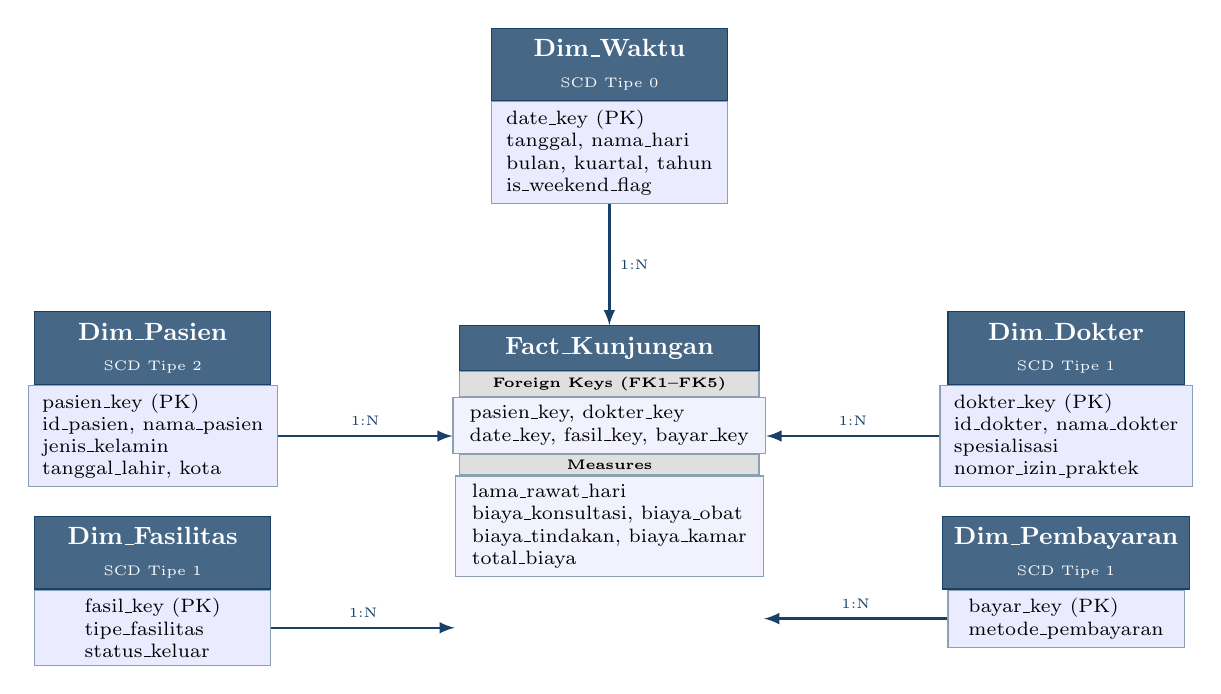
\begin{tikzpicture}[
    DH/.style={rectangle, draw=ugmblue, fill=ugmblue!80, text=white,
      font=\small\bfseries, align=center,
      minimum width=3.0cm, inner xsep=4pt, inner ysep=4pt},
    DB/.style={rectangle, draw=ugmblue!50, fill=blue!8,
      font=\scriptsize, align=flush left,
      minimum width=3.0cm, inner xsep=5pt, inner ysep=3pt},
    FH/.style={rectangle, draw=ugmblue, fill=ugmblue!80, text=white,
      font=\small\bfseries, align=center,
      minimum width=3.8cm, inner xsep=4pt, inner ysep=4pt},
    FB/.style={rectangle, draw=ugmblue!50, fill=blue!5,
      font=\scriptsize, align=flush left,
      minimum width=3.8cm, inner xsep=6pt, inner ysep=3pt},
    FS/.style={rectangle, draw=ugmblue!50, fill=gray!25,
      font=\tiny\bfseries, align=center,
      minimum width=3.8cm, inner xsep=4pt, inner ysep=2pt},
    arr/.style={->, >=latex, line width=0.9pt, color=ugmblue}
  ]
    %% Dim_Waktu (atas tengah)
    \node[DH] (wh) at (0,5.8) {Dim\_Waktu\\\normalfont\tiny SCD Tipe 0};
    \node[DB, below=0pt of wh] (wb)
      {date\_key (PK)\\tanggal, nama\_hari\\bulan, kuartal, tahun\\is\_weekend\_flag};

    %% Dim_Pasien (kiri)
    \node[DH] (ph) at (-5.8,2.2) {Dim\_Pasien\\\normalfont\tiny SCD Tipe 2};
    \node[DB, below=0pt of ph] (pb)
      {pasien\_key (PK)\\id\_pasien, nama\_pasien\\jenis\_kelamin\\tanggal\_lahir, kota};

    %% Dim_Dokter (kanan)
    \node[DH] (dkh) at (5.8,2.2) {Dim\_Dokter\\\normalfont\tiny SCD Tipe 1};
    \node[DB, below=0pt of dkh] (dkb)
      {dokter\_key (PK)\\id\_dokter, nama\_dokter\\spesialisasi\\nomor\_izin\_praktek};

    %% Dim_Fasilitas (kiri bawah) – naik sedikit
    \node[DH] (fsh) at (-5.8,-0.4) {Dim\_Fasilitas\\\normalfont\tiny SCD Tipe 1};
    \node[DB, below=0pt of fsh] (fsb)
      {fasil\_key (PK)\\tipe\_fasilitas\\status\_keluar};

    %% Dim_Pembayaran (kanan bawah) – naik sedikit
    \node[DH] (pyh) at (5.8,-0.4) {Dim\_Pembayaran\\\normalfont\tiny SCD Tipe 1};
    \node[DB, below=0pt of pyh] (pyb)
      {bayar\_key (PK)\\metode\_pembayaran};

    %% Fact_Kunjungan (tengah)
    \node[FH] (fch) at (0,2.2) {Fact\_Kunjungan};
    \node[FS, below=0pt of fch] (fcsk) {Foreign Keys (FK1--FK5)};
    \node[FB, below=0pt of fcsk] (fckb)
      {pasien\_key, dokter\_key\\date\_key, fasil\_key, bayar\_key};
    \node[FS, below=0pt of fckb] (fcsm) {Measures};
    \node[FB, below=0pt of fcsm] (fcmb)
      {lama\_rawat\_hari\\biaya\_konsultasi, biaya\_obat\\biaya\_tindakan, biaya\_kamar\\total\_biaya};

    %% Arrows
    \draw[arr] (wb.south)  -- (fch.north)          node[midway,right,font=\tiny]{1:N};
    \draw[arr] (pb.east)   -- (pb.east  -| fckb.west) node[midway,above,font=\tiny]{1:N};
    \draw[arr] (dkb.west)  -- (dkb.west -| fckb.east) node[midway,above,font=\tiny]{1:N};
    \draw[arr] (fsb.east)  -- (fsb.east -| fcmb.west) node[midway,above,font=\tiny]{1:N};
    \draw[arr] (pyb.west)  -- (pyb.west -| fcmb.east) node[midway,above,font=\tiny]{1:N};
  \end{tikzpicture}
  }
  \end{center}
\end{frame}

\begin{frame}{Arsitektur Staging dan Alur ETL}
  \footnotesize
  \begin{columns}[T]
    \column{0.50\textwidth}
    \textbf{Tiga Tabel Staging (Truncate \& Load)}
    \begin{itemize}
      \scriptsize
      \item \texttt{stg\_pasien} $\leftarrow$ \texttt{source\_pasien.csv}
      \item \texttt{stg\_dokter} $\leftarrow$ \texttt{source\_dokter.csv}
      \item \texttt{stg\_kunjungan} $\leftarrow$ \texttt{source\_kunjungan.csv}
    \end{itemize}

    \vspace{6pt}
    \textbf{Fungsi Staging Area}
    \begin{itemize}
      \scriptsize
      \item Ekstraksi cepat dari file CSV ke database
      \item Validasi dan penyelarasan format tipe data
      \item Pembentukan \textit{Surrogate Key}
    \end{itemize}

    \column{0.48\textwidth}
    \textbf{Alur Transformasi ke Star Schema}
    \vspace{6pt}

    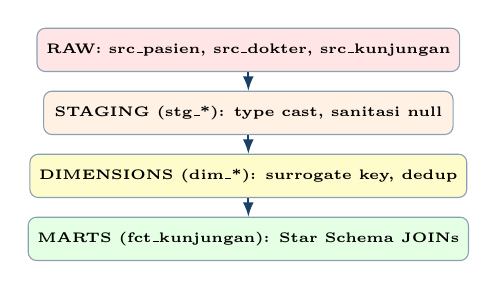
\begin{tikzpicture}[
      box/.style={rectangle, draw=ugmblue!50, rounded corners=3pt,
        minimum width=5.2cm, minimum height=0.55cm,
        align=center, font=\tiny\bfseries},
      arr/.style={->, >=latex, thick, color=ugmblue}
    ]
      \node[box, fill=red!10]    (raw) at (0,0)    {RAW: src\_pasien, src\_dokter, src\_kunjungan};
      \node[box, fill=orange!10] (stg) at (0,-0.8) {STAGING (stg\_*): type cast, sanitasi null};
      \node[box, fill=yellow!20] (dim) at (0,-1.6) {DIMENSIONS (dim\_*): surrogate key, dedup};
      \node[box, fill=green!10]  (mrt) at (0,-2.4) {MARTS (fct\_kunjungan): Star Schema JOINs};
      \draw[arr] (raw)--(stg); \draw[arr] (stg)--(dim); \draw[arr] (dim)--(mrt);
    \end{tikzpicture}

    \vspace{6pt}
    \begin{block}{}
      \tiny Orkestrasi pipeline menggunakan \textbf{Apache Airflow} dengan \textit{manual trigger}
    \end{block}
  \end{columns}
\end{frame}

%=============================================================
%  BAB 4: SYNTHETIC DATA GENERATION
%=============================================================
\section{Synthetic Data Generation}

\begin{frame}[fragile]{Strategi dan Aturan Generator Data Sintetis}
  \footnotesize
  \begin{columns}[T]
    \column{0.50\textwidth}
    \textbf{4 Constraint Enforcement (Python + Faker)}
    \begin{enumerate}
      \scriptsize
      \item \textbf{Sinergi Tarif Medis:} \texttt{biaya\_konsultasi} dikunci berdasarkan kamus tarif per spesialisasi dokter.
      \item \textbf{Isolasi Fasilitas Non-Inap:} IGD dan Rawat Jalan $\Rightarrow$ \texttt{lama\_rawat = 0}, \texttt{biaya\_kamar = 0}.
      \item \textbf{Pembobotan Status Keluar:} 80\% Sembuh, 12\% Dirujuk, 6\% Pulang Paksa, 2\% Meninggal (Rawat Inap).
      \item \textbf{Integritas Billing:} \texttt{total = konsultasi + obat + tindakan + kamar} (deterministik).
    \end{enumerate}

    \vspace{5pt}
    \begin{block}{Konfigurasi Volume}
      \scriptsize
      \begin{tabular}{@{}ll@{}}
        TOTAL\_PASIEN    & 2.500 \\
        TOTAL\_DOKTER    & 80 \\
        TOTAL\_KUNJUNGAN & 12.000 \\
        Seed             & \texttt{42} (reprodusibel) \\
      \end{tabular}
    \end{block}

    \column{0.48\textwidth}
    \textbf{Cuplikan Logika Generator}
    \begin{lstlisting}[language=Python]
# Logika Rawat Inap
if tipe_fasilitas == 'Rawat Inap':
    lama_rawat = random.randint(1, 14)
    status_keluar = random.choices(
        ['Sembuh','Dirujuk',
         'Pulang Paksa','Meninggal'],
        weights=[80, 12, 6, 2])[0]
    biaya_kamar = lama_rawat * \
        random.choice([250000,500000,
                       1200000])
else:
    lama_rawat    = 0
    status_keluar = 'Sembuh'
    biaya_kamar   = 0

# Billing deterministik
total_biaya = (biaya_konsul + biaya_obat
               + biaya_tindakan
               + biaya_kamar)
    \end{lstlisting}
  \end{columns}
\end{frame}

%=============================================================
%  BAB 5: IMPLEMENTASI APACHE AIRFLOW
%=============================================================
\section{Implementasi Orkestrasi Apache Airflow}

\begin{frame}{Arsitektur DAG dan Topologi Task}
  \footnotesize
  \begin{columns}[T]
    \column{0.46\textwidth}
    \textbf{DAG: \texttt{01\_healthcare\_data\_pipeline}}
    \vspace{4pt}

    \begin{block}{Parameter \textit{default args}}
      \scriptsize
      \begin{tabular}{@{}ll@{}}
        Owner           & \texttt{kelompok\_healthcare} \\
        Depends on Past & False \\
        Retries         & 1 kali \\
        Retry Delay     & 2 menit \\
        Schedule        & Manual Trigger \\
        Catchup         & False \\
      \end{tabular}
    \end{block}

    \vspace{5pt}
    \textbf{Alur Dependensi Sekuensial}
    \begin{tcolorbox}[
      colback=backcolour, colframe=ugmblue!50,
      top=2pt, bottom=2pt, left=4pt, right=4pt
    ]
      \tiny\ttfamily
      generate $\gg$ ingest $\gg$ auto\_dbt \\
      $\gg$ dbt\_run $\gg$ dbt\_test \\
      $\gg$ dbt\_docs $\gg$ dbt\_serve
    \end{tcolorbox}

    \column{0.52\textwidth}
    \textbf{7 Task Linear}
    \vspace{2pt}

    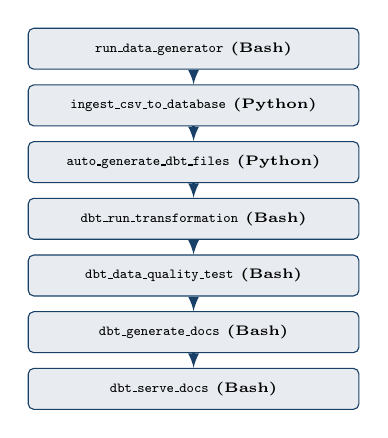
\begin{tikzpicture}[
      task/.style={rectangle, draw=ugmblue, rounded corners=2pt,
        fill=ugmblue!10, minimum width=4.2cm, minimum height=0.52cm,
        align=center, font=\tiny\bfseries},
      arr/.style={->, >=latex, thick, color=ugmblue}
    ]
      \node[task] (t1) at (0, 0)    {\texttt{run\_data\_generator} {\tiny(Bash)}};
      \node[task] (t2) at (0,-0.72) {\texttt{ingest\_csv\_to\_database} {\tiny(Python)}};
      \node[task] (t3) at (0,-1.44) {\texttt{auto\_generate\_dbt\_files} {\tiny(Python)}};
      \node[task] (t4) at (0,-2.16) {\texttt{dbt\_run\_transformation} {\tiny(Bash)}};
      \node[task] (t5) at (0,-2.88) {\texttt{dbt\_data\_quality\_test} {\tiny(Bash)}};
      \node[task] (t6) at (0,-3.60) {\texttt{dbt\_generate\_docs} {\tiny(Bash)}};
      \node[task] (t7) at (0,-4.32) {\texttt{dbt\_serve\_docs} {\tiny(Bash)}};
      \draw[arr] (t1)--(t2); \draw[arr] (t2)--(t3);
      \draw[arr] (t3)--(t4); \draw[arr] (t4)--(t5);
      \draw[arr] (t5)--(t6); \draw[arr] (t6)--(t7);
    \end{tikzpicture}
  \end{columns}
\end{frame}

\begin{frame}{Penjelasan Task 1--4}
  \footnotesize
  \begin{block}{Task 1: \texttt{run\_data\_generator} (BashOperator)}
    \scriptsize Menjalankan \texttt{generator.py} via shell. Menghasilkan 3 file CSV (\texttt{source\_pasien}, \texttt{source\_dokter}, \texttt{source\_kunjungan}) di direktori \textit{shared storage} sebelum task berikutnya berjalan.
  \end{block}
  \vspace{3pt}
  \begin{block}{Task 2: \texttt{ingest\_csv\_to\_database} (PythonOperator)}
    \scriptsize Fungsi \texttt{ingest\_csv\_to\_postgres()} membaca CSV via Pandas, menulis ke tabel \texttt{src\_*} di PostgreSQL. Strategi \textit{idempotent}: TRUNCATE lalu append jika tabel sudah ada, buat baru jika belum.
  \end{block}
  \vspace{3pt}
  \begin{block}{Task 3: \texttt{auto\_generate\_dbt\_files} (PythonOperator)}
    \scriptsize Fungsi \texttt{auto\_generate\_dbt\_models()} mengunduh manifest YAML dari GitHub, lalu secara otomatis membuat seluruh file \texttt{.sql} model dbt di folder \texttt{staging/}, \texttt{dimensions/}, \texttt{marts/} dan menghasilkan \texttt{sources.yml}.
  \end{block}
  \vspace{3pt}
  \begin{block}{Task 4: \texttt{dbt\_run\_transformation} (BashOperator)}
    \scriptsize Perintah \texttt{dbt run --target docker\_env} mengompilasi dan mengeksekusi seluruh model SQL, membangun Star Schema (tabel fakta dan dimensi) secara persisten di PostgreSQL.
  \end{block}
\end{frame}

\begin{frame}{Penjelasan Task 5--7}
  \footnotesize
  \begin{block}{Task 5: \texttt{dbt\_data\_quality\_test} (BashOperator)}
    \scriptsize Perintah \texttt{dbt test} menjalankan 30 aturan pengujian (\texttt{unique}, \texttt{not\_null}, \texttt{accepted\_values}, \texttt{relationships}). Jika ada pengujian gagal, Airflow menandai task \textcolor{red}{\textbf{Failed}} dan menghentikan seluruh pipeline sehingga data tidak valid tidak sampai ke laporan.
  \end{block}
  \vspace{4pt}
  \begin{block}{Task 6: \texttt{dbt\_generate\_docs} (BashOperator)}
    \scriptsize Perintah \texttt{dbt docs generate} mengompilasi seluruh metadata model, kolom, deskripsi, dan hasil pengujian menjadi artefak statis \texttt{manifest.json} dan \texttt{catalog.json} sebagai fondasi portal dokumentasi interaktif dbt.
  \end{block}
  \vspace{4pt}
  \begin{block}{Task 7: \texttt{dbt\_serve\_docs} (BashOperator)}
    \scriptsize Menjalankan server dokumentasi di \textit{background} via \texttt{nohup dbt docs serve --port 8081 \&}. Port 8081 dibersihkan terlebih dahulu (\texttt{fuser -k}) sebelum server baru dijalankan sebagai \textit{daemon}. Dokumentasi dapat diakses di \texttt{http://localhost:8081}.
  \end{block}
\end{frame}

%=============================================================
%  BAB 6: IMPLEMENTASI DBT
%=============================================================
\section{Implementasi dbt (Data Build Tool)}

\begin{frame}{Peran dbt dan Struktur Proyek}
  \footnotesize
  \begin{columns}[T]
    \column{0.46\textwidth}
    \textbf{Pendekatan ELT (bukan ETL)}
    \vspace{4pt}

    Setelah data mentah dimuat oleh Airflow, seluruh transformasi diserahkan ke \textbf{dbt} dengan keunggulan:
    \begin{itemize}
      \scriptsize
      \item Transformasi SQL modular dan versi-terkontrol
      \item \textit{Layering} logika bisnis yang terpisah
      \item Pengujian integritas otomatis
      \item Dokumentasi skema interaktif
    \end{itemize}

    \vspace{6pt}
    \textbf{Konfigurasi Materialisasi}
    \begin{itemize}
      \scriptsize
      \item \texttt{staging/} $\Rightarrow$ \textbf{view} (hemat storage)
      \item \texttt{dimensions/} $\Rightarrow$ \textbf{table} (fisik)
      \item \texttt{marts/} $\Rightarrow$ \textbf{table} (fisik, cepat)
    \end{itemize}

    \column{0.52\textwidth}
    \textbf{Struktur Direktori \texttt{dbt\_project/}}
    \begin{itemize}
      \scriptsize
      \item[\texttt{-}] \texttt{dbt\_project.yml} --- konfigurasi utama
      \item[\texttt{-}] \texttt{profiles.yml} --- kredensial PostgreSQL
      \item[\texttt{-}] \texttt{models/staging/}
        \begin{itemize}\tiny
          \item \texttt{stg\_pasien.sql}, \texttt{stg\_dokter.sql}
          \item \texttt{stg\_kunjungan.sql}, \texttt{sources.yml}
        \end{itemize}
      \item[\texttt{-}] \texttt{models/dimensions/}
        \begin{itemize}\tiny
          \item \texttt{dim\_pasien.sql}, \texttt{dim\_dokter.sql}
          \item \texttt{dim\_waktu.sql}, \texttt{dim\_fasilitas.sql}
          \item \texttt{dim\_pembayaran.sql}
        \end{itemize}
      \item[\texttt{-}] \texttt{models/marts/}
        \begin{itemize}\tiny
          \item \texttt{fct\_kunjungan.sql} --- tabel fakta utama
          \item \texttt{schema.yml} --- pengujian \& dokumentasi
        \end{itemize}
    \end{itemize}
  \end{columns}
\end{frame}

\begin{frame}{Arsitektur Lapisan dbt dan Data Lineage}
  \footnotesize
  \begin{columns}[T]
    \column{0.48\textwidth}
    \textbf{3 Lapisan Transformasi}
    \vspace{4pt}

    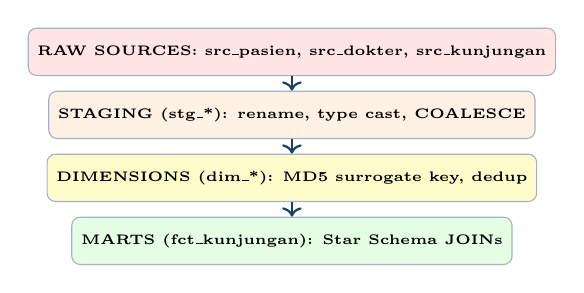
\begin{tikzpicture}[
      layer/.style={rectangle, draw=ugmblue!40, rounded corners=3pt,
        minimum width=5.2cm, minimum height=0.6cm,
        align=center, font=\tiny\bfseries},
      arr/.style={->, thick, color=ugmblue}
    ]
      \node[layer, fill=red!10]    (raw) at (0,0)    {RAW SOURCES: src\_pasien, src\_dokter, src\_kunjungan};
      \node[layer, fill=orange!10] (stg) at (0,-0.8) {STAGING (stg\_*): rename, type cast, COALESCE};
      \node[layer, fill=yellow!20] (dim) at (0,-1.6) {DIMENSIONS (dim\_*): MD5 surrogate key, dedup};
      \node[layer, fill=green!10]  (mrt) at (0,-2.4) {MARTS (fct\_kunjungan): Star Schema JOINs};
      \draw[arr] (raw)--(stg); \draw[arr] (stg)--(dim); \draw[arr] (dim)--(mrt);
    \end{tikzpicture}

    \column{0.50\textwidth}
    \textbf{Lapisan Staging}
    \begin{itemize}
      \scriptsize
      \item Standardisasi nama kolom (snake\_case)
      \item Penyelarasan tipe data (\texttt{NUMERIC(15,2)})
      \item Sanitasi null values dengan \texttt{COALESCE}
    \end{itemize}

    \textbf{Lapisan Dimensions}
    \begin{itemize}
      \scriptsize
      \item \textit{Surrogate Key} berbasis MD5 hash
      \item Deduplication via \texttt{ROW\_NUMBER()}
      \item Ekspansi dimensi waktu (hari, bulan, kuartal, tahun)
    \end{itemize}

    \textbf{Lapisan Marts}
    \begin{itemize}
      \scriptsize
      \item Star Schema JOINs lintas dimensi
      \item Substitusi \textit{natural key} ke \textit{surrogate key}
      \item Isolasi \textit{additive measures} (6 kolom numerik)
    \end{itemize}

    \begin{block}{}
      \tiny \textbf{dbt Docs} (port 8081): \textit{Data Lineage Graph} interaktif dari sumber hingga \texttt{fct\_kunjungan}
    \end{block}
  \end{columns}
\end{frame}

%=============================================================
%  BAB 7: PEMBANGUNAN DATA MART
%=============================================================
\section{Pembangunan Data Mart}

\begin{frame}{Skema Final Data Mart dan Koneksi BI}
  \footnotesize
  \begin{columns}[T]
    \column{0.52\textwidth}
    \begin{block}{Tabel Fakta: \texttt{fct\_kunjungan}}
      \tiny
      \begin{tabular}{@{}lll@{}}
        \toprule
        \textbf{Kolom} & \textbf{Peran} & \textbf{Tipe} \\
        \midrule
        \texttt{kunjungan\_key}   & PK      & VARCHAR(50)   \\
        \texttt{pasien\_key}      & FK      & INT           \\
        \texttt{dokter\_key}      & FK      & INT           \\
        \texttt{waktu\_key}       & FK      & INT           \\
        \texttt{fasilitas\_key}   & FK      & VARCHAR(50)   \\
        \texttt{pembayaran\_key}  & FK      & VARCHAR(50)   \\
        \texttt{durasi\_rawat}    & Measure & INT           \\
        \texttt{biaya\_konsultasi}& Measure & NUMERIC(15,2) \\
        \texttt{biaya\_obat}      & Measure & NUMERIC(15,2) \\
        \texttt{biaya\_tindakan}  & Measure & NUMERIC(15,2) \\
        \texttt{biaya\_kamar}     & Measure & NUMERIC(15,2) \\
        \texttt{total\_biaya}     & Calc.   & NUMERIC(15,2) \\
        \bottomrule
      \end{tabular}
    \end{block}

    \column{0.46\textwidth}
    \textbf{Koneksi Metabase (BI Tool)}
    \vspace{4pt}

    \scriptsize
    \begin{tabular}{@{}ll@{}}
      \toprule
      \textbf{Parameter} & \textbf{Nilai} \\
      \midrule
      Database Type & PostgreSQL \\
      Nama          & \texttt{healthcare\_01} \\
      Host          & \texttt{host.docker.internal} \\
      Port          & \texttt{5555} \\
      Database      & \texttt{airflow} \\
      Username      & \texttt{airflow} \\
      Schemas       & All \\
      \bottomrule
    \end{tabular}
  \end{columns}
\end{frame}

\begin{frame}{Skema Final Data Mart dan Koneksi BI}
  \footnotesize
  \begin{columns}[T]
    \column{0.52\textwidth}
        \vspace{5pt}
    \begin{block}{Port Forwarding}
      \tiny Port \texttt{5555} dipakai karena Metabase mengakses PostgreSQL dari luar Docker, via pemetaan \texttt{5555:5432} di \texttt{docker-compose.yaml}.
    \end{block}
    \column{0.46\textwidth}
    \vspace{4pt}
    \textbf{Semantic Layer}
    \tiny
    \begin{align*}
      \text{Total Biaya}     &= \text{Konsultasi} + \text{Obat} + \text{Tindakan} + \text{Kamar} \\
      \text{Avg LoS}         &= \text{AVG}(\texttt{durasi\_rawat}) \\
      \text{Total Kunjungan} &= \text{COUNT}(\texttt{kunjungan\_key})
    \end{align*}
  \end{columns}
\end{frame}
%=============================================================
%  BAB 8: VERIFIKASI DAN VALIDASI
%=============================================================
\section{Verifikasi dan Validasi Data Mart}

% %--- Slide BQ-01 dan BQ-02 ---
% \begin{frame}[fragile]{Query Analitik (BQ-01 \& BQ-02)}
%   \footnotesize
%   \begin{block}{BQ-01: Total Pendapatan per Tipe Fasilitas}
%     \begin{lstlisting}[language=SQL]
% SELECT f.tipe_fasilitas,
%        COUNT(fk.pasien_key) AS jumlah_kunjungan,
%        SUM(fk.total_biaya)  AS total_pendapatan,
%        ROUND(SUM(fk.total_biaya)*100.0
%              /SUM(SUM(fk.total_biaya)) OVER(),2) AS persen_kontribusi
% FROM fact_kunjungan fk
% JOIN dim_fasilitas f ON fk.fasilitas_key=f.fasilitas_key
% GROUP BY f.tipe_fasilitas ORDER BY total_pendapatan DESC;
%     \end{lstlisting}
%   \end{block}
%   \vspace{4pt}
%   \begin{block}{BQ-02: Kinerja Dokter per Spesialisasi (Top 5)}
%     \begin{lstlisting}[language=SQL]
% SELECT d.spesialisasi,
%        COUNT(fk.kunjungan_key)         AS total_kunjungan,
%        SUM(fk.total_biaya)             AS total_pendapatan,
%        ROUND(AVG(fk.biaya_konsultasi),2) AS avg_biaya_konsultasi
% FROM fct_kunjungan fk
% JOIN dim_dokter d ON fk.dokter_key=d.dokter_key
% GROUP BY d.spesialisasi ORDER BY total_kunjungan DESC LIMIT 5;
%     \end{lstlisting}
%   \end{block}
% \end{frame}

% %--- Slide BQ-03 dan BQ-04 ---
% \begin{frame}[fragile]{Query Analitik (BQ-03 \& BQ-04)}
%   \footnotesize
%   \vspace{-2pt}
%   \begin{block}{BQ-03: Distribusi Metode Pembayaran}
%     \begin{lstlisting}[language=SQL]
% SELECT pb.metode_pembayaran,
%        COUNT(fk.pasien_key) AS jumlah_transaksi,
%        SUM(fk.total_biaya)  AS total_biaya_pelayanan,
%        ROUND(COUNT(fk.pasien_key)*100.0
%              /SUM(COUNT(fk.pasien_key)) OVER(),2) AS persen_transaksi,
%        ROUND(SUM(fk.total_biaya)*100.0
%              /SUM(SUM(fk.total_biaya)) OVER(),2)  AS persen_biaya
% FROM fact_kunjungan fk
% JOIN dim_pembayaran pb ON fk.bayar_key=pb.bayar_key
% GROUP BY pb.metode_pembayaran ORDER BY total_biaya_pelayanan DESC;
%     \end{lstlisting}
%   \end{block}
%   \vspace{-2pt}
%   \begin{block}{BQ-04: Analisis Length of Stay (LOS)}
%     \begin{lstlisting}[language=SQL]
% SELECT CASE WHEN lama_rawat_hari=0 THEN '0 hari (non-inap)'
%             WHEN lama_rawat_hari BETWEEN 1 AND 3 THEN '1-3 hari'
%             WHEN lama_rawat_hari BETWEEN 4 AND 7 THEN '4-7 hari'
%             ELSE '8-14 hari' END AS kategori_los,
%        COUNT(pasien_key)              AS jumlah_kunjungan,
%        ROUND(AVG(lama_rawat_hari),2)  AS avg_los,
%        ROUND(AVG(biaya_kamar),2)      AS avg_biaya_kamar,
%        ROUND(AVG(total_biaya),2)      AS avg_total_biaya
% FROM fact_kunjungan GROUP BY kategori_los ORDER BY MIN(lama_rawat_hari);
%     \end{lstlisting}
%   \end{block}
% \end{frame}

% %--- Slide BQ-05---
% \begin{frame}[fragile]{Query Analitik (BQ-05)}
%   \footnotesize
%   \begin{block}{BQ-05: Tren Bulanan Volume Kunjungan}
%     \begin{lstlisting}[language=SQL]
% SELECT w.tahun, w.bulan,
%        COUNT(fk.pasien_key) AS jumlah_kunjungan,
%        SUM(fk.total_biaya)  AS total_pendapatan,
%        LAG(COUNT(fk.pasien_key)) OVER (ORDER BY w.tahun,w.bulan)
%          AS kunjungan_bulan_sebelumnya,
%        ROUND((COUNT(fk.pasien_key)
%               - LAG(COUNT(fk.pasien_key)) OVER (ORDER BY w.tahun,w.bulan))
%              *100.0 / NULLIF(LAG(COUNT(fk.pasien_key))
%              OVER (ORDER BY w.tahun,w.bulan),0),2) AS persen_pertumbuhan
% FROM fact_kunjungan fk
% JOIN dim_waktu w ON fk.date_key=w.date_key
% GROUP BY w.tahun,w.bulan ORDER BY w.tahun,w.bulan;
%     \end{lstlisting}
%   \end{block}
% \end{frame}

% %--- Slide BQ-06 ---
% \begin{frame}[fragile]{Query Analitik (BQ-06)}
%   \footnotesize

%   \begin{block}{BQ-06: Proporsi Status Keluar Pasien Rawat Inap}
%     \begin{lstlisting}[language=SQL]
% SELECT f.status_keluar,
%        COUNT(fk.pasien_key)          AS jumlah_pasien,
%        ROUND(AVG(fk.lama_rawat_hari),2) AS avg_lama_rawat,
%        ROUND(AVG(fk.total_biaya),2)     AS avg_total_biaya,
%        ROUND(COUNT(fk.pasien_key)*100.0
%              /SUM(COUNT(fk.pasien_key)) OVER(),2) AS persen_proporsi
% FROM fact_kunjungan fk
% JOIN dim_fasilitas f ON fk.fasilitas_key=f.fasilitas_key
% WHERE f.tipe_fasilitas = 'Rawat Inap'
% GROUP BY f.status_keluar ORDER BY jumlah_pasien DESC;
%     \end{lstlisting}
%   \end{block}
% \end{frame}

% %--- Slide BQ-07 dan BQ-08 ---
% \begin{frame}[fragile]{Query Analitik (BQ-07 \& BQ-08)}
%   \footnotesize
%   \vspace{-6pt}
%   \begin{block}{BQ-07: Breakdown Kontribusi Komponen Biaya}
%     \begin{lstlisting}[language=SQL]
% WITH komponen AS (
%   SELECT 'Konsultasi' AS k, SUM(biaya_konsultasi) AS total,
%          ROUND(AVG(biaya_konsultasi),2) AS rata FROM fact_kunjungan
%   UNION ALL SELECT 'Obat',     SUM(biaya_obat),     ROUND(AVG(biaya_obat),2)     FROM fact_kunjungan
%   UNION ALL SELECT 'Tindakan', SUM(biaya_tindakan), ROUND(AVG(biaya_tindakan),2) FROM fact_kunjungan
%   UNION ALL SELECT 'Kamar',    SUM(biaya_kamar),    ROUND(AVG(biaya_kamar),2)    FROM fact_kunjungan
% )
% SELECT k AS komponen, total, rata,
%        ROUND(total*100.0/SUM(total) OVER(),2) AS persen_kontribusi
% FROM komponen ORDER BY total DESC;
%     \end{lstlisting}
%   \end{block}
%   \vspace{-4pt}
%   \begin{block}{BQ-08: Distribusi Kunjungan per Kota Asal Pasien (Top 10)}
%     \begin{lstlisting}[language=SQL]
% SELECT p.kota,
%        COUNT(fk.pasien_key)           AS jumlah_kunjungan,
%        COUNT(DISTINCT p.pasien_key)   AS jumlah_pasien_unik,
%        SUM(fk.total_biaya)            AS total_biaya,
%        ROUND(AVG(fk.total_biaya),2)   AS avg_biaya_per_kunjungan,
%        ROUND(COUNT(fk.pasien_key)*100.0
%              /SUM(COUNT(fk.pasien_key)) OVER(),2) AS persen_kunjungan
% FROM fact_kunjungan fk
% JOIN dim_pasien p ON fk.pasien_key=p.pasien_key
% GROUP BY p.kota ORDER BY jumlah_kunjungan DESC LIMIT 10;
%     \end{lstlisting}
%   \end{block}
% \end{frame}

% %--- Slide BQ-09 dan BQ-10 ---
% \begin{frame}[fragile]{Query Analitik (BQ-09)}
%   \footnotesize
%   \begin{block}{BQ-09: Profil Demografi (Jenis Kelamin x Golongan Darah)}
%     \begin{lstlisting}[language=SQL]
% SELECT p.jenis_kelamin, p.golongan_darah,
%        COUNT(fk.pasien_key)       AS jumlah_kunjungan,
%        ROUND(AVG(fk.total_biaya),2)  AS avg_biaya,
%        ROUND(COUNT(fk.pasien_key)*100.0
%              /SUM(COUNT(fk.pasien_key)) OVER(),2) AS persen_total,
%        ROUND(COUNT(fk.pasien_key)*100.0
%              /SUM(COUNT(fk.pasien_key))
%               OVER(PARTITION BY p.jenis_kelamin),2) AS persen_per_gender
% FROM fact_kunjungan fk
% JOIN dim_pasien p ON fk.pasien_key=p.pasien_key
% GROUP BY p.jenis_kelamin, p.golongan_darah
% ORDER BY p.jenis_kelamin, jumlah_kunjungan DESC;
%     \end{lstlisting}
%   \end{block}
% \end{frame}

% \begin{frame}[fragile]{Query Analitik (BQ-10)}
%   \footnotesize
%   \begin{block}{BQ-10: Komparasi Rata-Rata Biaya Obat IGD vs.\ Rawat Jalan}
%     \begin{lstlisting}[language=SQL]
% SELECT f.tipe_fasilitas,
%        COUNT(fk.pasien_key)           AS jumlah_kunjungan,
%        ROUND(AVG(fk.biaya_obat),2)    AS avg_biaya_obat,
%        ROUND(MIN(fk.biaya_obat),2)    AS min_biaya_obat,
%        ROUND(MAX(fk.biaya_obat),2)    AS max_biaya_obat,
%        ROUND(STDDEV(fk.biaya_obat),2) AS standar_deviasi,
%        ROUND(AVG(fk.biaya_obat)*100.0
%              /NULLIF(AVG(fk.total_biaya),0),2) AS persen_thd_total
% FROM fact_kunjungan fk
% JOIN dim_fasilitas f ON fk.fasilitas_key=f.fasilitas_key
% WHERE f.tipe_fasilitas IN ('IGD','Rawat Jalan')
% GROUP BY f.tipe_fasilitas ORDER BY avg_biaya_obat DESC;
%     \end{lstlisting}
%   \end{block}
% \end{frame}

% %--- Slide BQ-11 ---
% \begin{frame}[fragile]{Query Analitik (BQ-11)}
%   \footnotesize
%   \begin{block}{BQ-11: Peringkat Top 5 Dokter Teraktif}
%     \begin{lstlisting}[language=SQL]
% SELECT d.nama_dokter, d.spesialisasi, d.nomor_izin_praktek,
%        COUNT(fk.pasien_key)          AS jumlah_kunjungan,
%        SUM(fk.total_biaya)           AS total_pendapatan,
%        ROUND(AVG(fk.total_biaya),2)  AS avg_biaya_per_kunjungan,
%        ROUND(AVG(fk.lama_rawat_hari),2) AS avg_lama_rawat,
%        RANK() OVER (ORDER BY COUNT(fk.pasien_key) DESC) AS ranking
% FROM fact_kunjungan fk
% JOIN dim_dokter d ON fk.dokter_key=d.dokter_key
% GROUP BY d.nama_dokter, d.spesialisasi, d.nomor_izin_praktek
% ORDER BY jumlah_kunjungan DESC LIMIT 5;
%     \end{lstlisting}
%   \end{block}
% \end{frame}

% %--- Slide BQ-12 ---
% \begin{frame}[fragile]{Query Analitik (BQ-12)}
%   \footnotesize
%   \vspace{4pt}
%   \begin{block}{BQ-12: Average Ticket Size per Transaksi Kunjungan}
%     \begin{lstlisting}[language=SQL]
% SELECT COUNT(*)                                          AS total_transaksi,
%        ROUND(AVG(total_biaya)::numeric,2)                AS avg_ticket_size,
%        ROUND(MIN(total_biaya)::numeric,2)                AS minimum,
%        ROUND(MAX(total_biaya)::numeric,2)                AS maksimum,
%        ROUND(STDDEV(total_biaya)::numeric,2)             AS standar_deviasi,
%        ROUND(PERCENTILE_CONT(0.25) WITHIN GROUP
%              (ORDER BY total_biaya)::numeric,2)          AS kuartil_1,
%        ROUND(PERCENTILE_CONT(0.50) WITHIN GROUP
%              (ORDER BY total_biaya)::numeric,2)          AS median,
%        ROUND(PERCENTILE_CONT(0.75) WITHIN GROUP
%              (ORDER BY total_biaya)::numeric,2)          AS kuartil_3
% FROM fact_kunjungan;
%     \end{lstlisting}
%   \end{block}
% \end{frame}

\begin{frame}{Hasil dbt Test: 30/30 PASS}
  \footnotesize
  \begin{columns}[T]
    \column{0.48\textwidth}
    \textbf{Metadata Eksekusi (26 Mei 2026, 23:02 UTC)}
    \vspace{4pt}

    \scriptsize
    \begin{tabular}{@{}ll@{}}
      \toprule
      \textbf{Parameter} & \textbf{Nilai} \\
      \midrule
      Versi dbt   & 1.8.0 (postgres=1.8.0) \\
      Target      & \texttt{docker\_env} \\
      Konkurensi  & 4 threads paralel \\
      Cakupan     & 9 model, 30 data tests \\
      Total Waktu & 2,23 detik \\
      \midrule
      \textbf{PASS}  & \textbf{30} \\
      WARN           & 0 \\
      ERROR          & 0 \\
      TOTAL          & 30 \\
      \bottomrule
    \end{tabular}

    \vspace{6pt}
    \begin{block}{{Kesimpulan}}
      \scriptsize Seluruh lapisan Star Schema bebas anomali data dan memiliki integritas referensial yang solid.
    \end{block}

    \column{0.50\textwidth}
    \textbf{Distribusi 30 Pengujian per Lapisan}
    \vspace{4pt}

    \scriptsize
    \begin{tabular}{@{}llll@{}}
      \toprule
      \textbf{Lapisan} & \textbf{Tipe Uji} & \textbf{Model} & \textbf{N} \\
      \midrule
      \multirow{3}{*}{Staging}
        & accepted\_values & stg\_pasien & 1 \\
        & not\_null        & stg\_*      & 5 \\
        & unique           & stg\_*      & 3 \\
      \midrule
      \multirow{2}{*}{Dimensi}
        & not\_null & dim\_* & 5 \\
        & unique    & dim\_* & 5 \\
      \midrule
      \multirow{2}{*}{Fakta}
        & not\_null     & fct\_* & 6 \\
        & relationships & fct\_* & 5 \\
      \midrule
      \multicolumn{3}{@{}l}{\textbf{Total}} & \textbf{30} \\
      \bottomrule
    \end{tabular}
  \end{columns}
\end{frame}

\begin{frame}{Hasil dbt Test: 30/30 PASS}
  \footnotesize
  \begin{columns}[T]
    \column{0.50\textwidth}
    \vspace{4pt}
    \textbf{Data Quality Check (4/4 PASS)}
    \begin{itemize}
      \scriptsize
      \item \textbf{Completeness:} 0 NULL pada semua FK dan measures
      \item \textbf{Validity:} 0 nilai \texttt{total\_biaya} negatif
      \item \textbf{Consistency:} hanya 3 kategori fasilitas valid
      \item \textbf{Row Count:} 12.000 baris (selisih = 0)
    \end{itemize}
  \end{columns}
\end{frame}
%=============================================================
%  BAB 9: KESIMPULAN
%=============================================================
\section{Kesimpulan dan Rekomendasi}

\begin{frame}{Ringkasan Pencapaian dan Tantangan}
  \footnotesize
  \begin{columns}[T]
    \column{0.52\textwidth}
    \textbf{Pencapaian Proyek (End-to-End)}
    \begin{enumerate}
      \scriptsize
      \item \textbf{Data Generator} --- 12.000 transaksi sintetis (Python + Faker, logika kondisional)
      \item \textbf{Pipeline Otomatis} --- DAG Airflow 7 task, return code 0
      \item \textbf{Transformasi dbt} --- 9 model SQL modular (3 staging, 5 dimensi, 1 fakta)
      \item \textbf{Data Mart} --- Star Schema terhubung ke Metabase, 12 BQ terjawab
      \item \textbf{Validasi} --- 30/30 dbt test PASS, 4/4 data quality check PASS
    \end{enumerate}

    \column{0.46\textwidth}
    \textbf{5 Tantangan Teknis}
    \begin{enumerate}
      \scriptsize
      \item \textbf{Port Forwarding Docker} --- solusi: \texttt{host.docker.internal:5555}
      \item \textbf{Surrogate Key inkonsisten} --- diseragamkan via \texttt{dbt\_utils.generate\_surrogate\_key()}
      \item \textbf{Distribusi data sintetis} --- logika \texttt{if-else} per tipe fasilitas
      \item \textbf{Dependensi task Airflow} --- operator \texttt{>>} + sensor task
      \item \textbf{Format tanggal lintas sistem} --- \texttt{pd.to\_datetime().dt.date} + \texttt{CAST(... AS DATE)}
    \end{enumerate}
  \end{columns}
\end{frame}

\begin{frame}{Keputusan Desain Utama}
  \scriptsize
  \begin{tabular}{@{}p{2.8cm}p{2.8cm}p{6.8cm}@{}}
    \toprule
    \textbf{Keputusan} & \textbf{Alternatif} & \textbf{Alasan Pemilihan} \\
    \midrule
    \textit{Star Schema} murni
      & \textit{Snowflake Schema}
      & Meminimalkan kompleksitas JOIN, mempercepat agregasi BI, mudah dipahami pengguna bisnis \\[3pt]
    Pendekatan ELT
      & ETL tradisional
      & Memanfaatkan kekuatan komputasi PostgreSQL; dbt mengelola transformasi secara versi-terkontrol \\[3pt]
    \textit{Surrogate Key} MD5
      & Auto-increment SERIAL
      & Deterministik dan reprodusibel saat pipeline diulang, mencegah duplikasi kunci \\[3pt]
    \texttt{view} untuk staging
      & \texttt{table} semua lapisan
      & Menghemat penyimpanan; staging bukan repositori permanen \\[3pt]
    Manual trigger Airflow
      & \texttt{@daily} otomatis
      & Kontrol eksplisit selama fase pengembangan \\[3pt]
    Data sintetis rule-based
      & GAN / VAE generatif
      & Lebih mudah dikontrol, reprodusibel via \texttt{seed(42)}, tidak butuh data latih \\
    \bottomrule
  \end{tabular}
\end{frame}

\begin{frame}{Kesiapan Data Mart untuk Visualisasi BI}
  \footnotesize
  \begin{columns}[T]
    \column{0.50\textwidth}
    \textbf{Checklist Kesiapan (7/7 Terpenuhi)}
    \vspace{4pt}

    \scriptsize
    \begin{tabular}{@{}clc@{}}
      \toprule
      \textbf{No} & \textbf{Kriteria} & \textbf{Status} \\
      \midrule
      1 & Integritas referensial antar tabel    & \tekshijau{\checkmark} \\
      2 & Tidak ada null pada kunci \& measures & \tekshijau{\checkmark} \\
      3 & Volume data 12.000 transaksi          & \tekshijau{\checkmark} \\
      4 & Koneksi Metabase berhasil             & \tekshijau{\checkmark} \\
      5 & Query analitik 12 BQ valid            & \tekshijau{\checkmark} \\
      6 & Star Schema terdeteksi Metabase       & \tekshijau{\checkmark} \\
      7 & Metrik KPI pada Semantic Layer        & \tekshijau{\checkmark} \\
      \bottomrule
    \end{tabular}

    \column{0.48\textwidth}
    \textbf{Rencana Dasbor Metabase}
    \begin{itemize}
      \scriptsize
      \item \textbf{Finansial:} Pendapatan per fasilitas, pie chart pembayaran, KPI total
      \item \textbf{Kinerja Klinis:} Ranking dokter, status keluar, avg LOS
      \item \textbf{Tren Operasional:} Tren bulanan kunjungan, breakdown biaya
      \item \textbf{Demografi:} Distribusi kota asal, cross-tab jenis kelamin x golongan darah
    \end{itemize}
  \end{columns}

  \vspace{4pt}
  \begin{tcolorbox}[
    colback=ugmblue!8, colframe=ugmblue,
    leftrule=4pt, toprule=0.4pt, bottomrule=0.4pt, rightrule=0.4pt,
    top=3pt, bottom=3pt, left=6pt, right=6pt
  ]
    \scriptsize\textbf{Kesimpulan Akhir:} Sistem DWBI operasional rumah sakit berhasil dibangun \textit{end-to-end}: integritas data terjamin, pipeline terotomatisasi, dokumentasi lengkap, dan Data Mart terhubung ke BI tool.
  \end{tcolorbox}
\end{frame}

%-------------------------------------------------------------
% PENUTUP
%-------------------------------------------------------------
\begin{frame}{}
  \begin{center}
    \vspace{0.8cm}
    {\Large\bfseries\color{ugmblue} Terima Kasih}

    \vspace{0.8cm}
    \scriptsize
    \begin{tabular}{@{}ll@{}}
      \textbf{Repository:}            & \url{https://github.com/vickymahfudy/dwbi-healthcare} \\[5pt]
      \textbf{Demo:}            & \url{https://drive.google.com/file/d/1wSzZUH0q-3eZJ2lBEaPGWqBdXCuA-ZFi/view} \\[5pt]
      \textbf{Engelbertus Rande}      & NIM 25/573149/PPA/07211 \\
      \textbf{Gilbert Fandiliam Mooy} & NIM 25/574767/PPA/07259 \\
      \textbf{Sinta Siti Nuriah}      & NIM 25/575177/PPA/07274 \\
      \textbf{Vicky Mahfudy}          & NIM 25/573019/PPA/07207 \\[6pt]
      \textbf{Dosen:}   & Khabib Mustofa \\
      \textbf{Program:} & S2 Ilmu Komputer, Universitas Gadjah Mada \\
    \end{tabular}

    \vspace{0.8cm}
    {\scriptsize\color{ugmblue}\textit{Data Warehouse and Business Intelligence --- Tugas Kelompok 2025/2026}}
  \end{center}
\end{frame}

%=============================================================
\end{document}
%=============================================================